\documentclass[usenames,dvipsnames,tikz]{standalone}
\usetikzlibrary{shapes.geometric}
%\usepackage{xcolor}
\colorlet{tBlue}{RoyalBlue!35!Cerulean}
\colorlet{tRed}{Red}
%\usepackage{tikz}
%\usepackage{standalone}
\begin{document}
	
% SUB-MSCPP MATCHING GRAPH
	
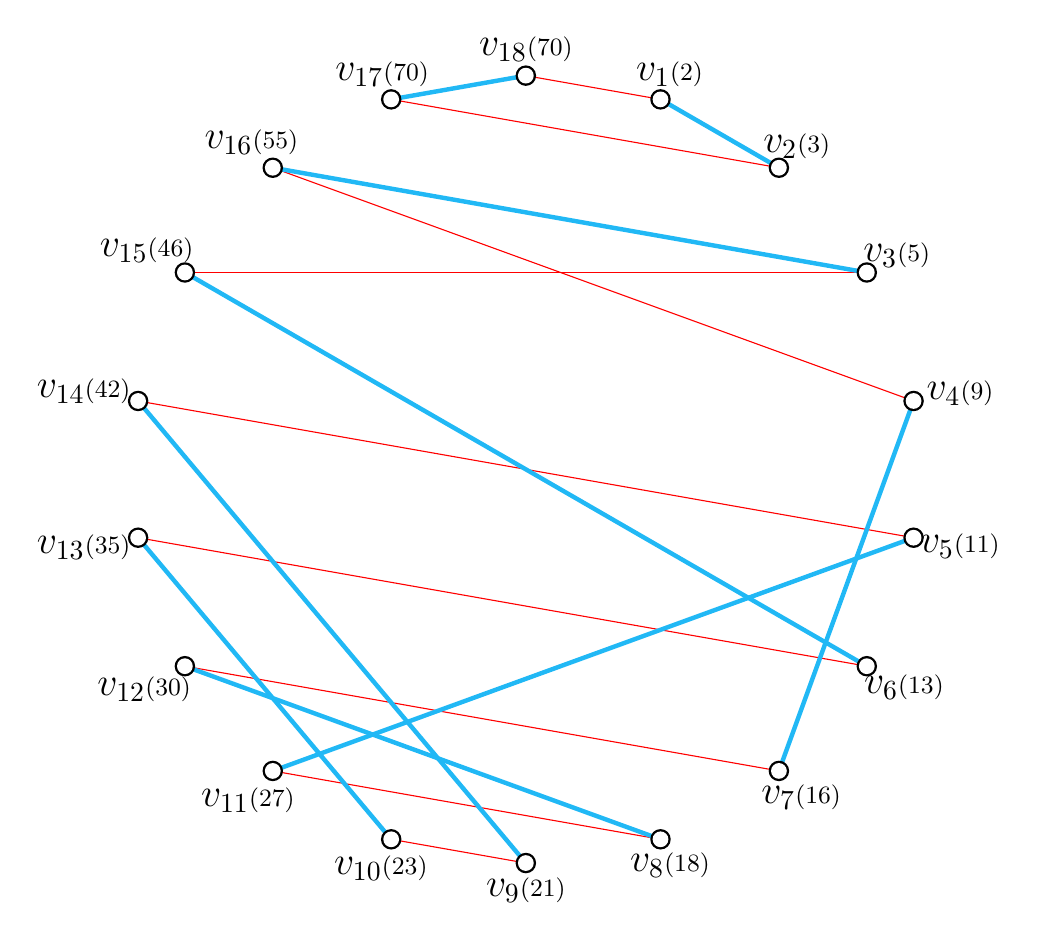
\begin{tikzpicture}
%Values of vertices:
% v1=2, v2=3, v3=5, v4=9, v5=11, v6=13, v7=16, v8=18, v9=21, v10=23, v11=27, v12=30, v13=35, v14=42, v15=46, v16=55, v17=70, v18=70 (v17/v18 universal vertices), \tau = 70.

%partners: v1-v2, v3-v16, v4-v7, v5-v11, v6-v15, v8-v12, v9-v14, v10-v13, v17-v18.


\foreach \n/\value in {1/1, 2/1, 3/2, 4/2, 5/3, 6/4, 7/4, 8/5, 9/5, 10/6, 11/6, 12/6, 13/6, 14/7, 15/8, 16/9, 17/10, 18/10}
	\fill (90-\n*20:5cm) coordinate (v\n) circle [radius = 0.1];
	
\foreach \n/\value in {1/2, 17/70, 18/70}
	\fill (90-\n*20:5cm) coordinate (v\n) circle [radius = 0.1]
		++(90-\n*20:9.5pt) node {\Large{$v_{\n}$}\small{($\value$)}};

\foreach \n/\value in {2/3, 8/18, 9/21}
	\fill (90-\n*20:5cm) coordinate (v\n) circle [radius = 0.1]
		++(90-\n*20:10pt) node {\Large{$v_{\n}$}\small{($\value$)}};
		
\foreach \n/\value in {3/5, 7/16}
	\fill (90-\n*20:5cm) coordinate (v\n) circle [radius = 0.1]
		++(90-\n*20:12.5pt) node {\Large{$v_{\n}$}\small{($\value$)}};		
		
\foreach \n/\value in {4/9, 5/11, 12/30}
	\fill (90-\n*20:5cm) coordinate (v\n) circle [radius = 0.1]
		++(90-\n*20:17pt) node {\Large{$v_{\n}$}\small{($\value$)}};

\foreach \n/\value in {15/46}
	\fill (90-\n*20:5cm) coordinate (v\n) circle [radius = 0.1]
		++(90-\n*20:16pt) node {\Large{$v_{\n}$}\small{($\value$)}};
	
\foreach \n/\value in {6/13}
	\fill (90-\n*20:5cm) coordinate (v\n) circle [radius = 0.1]
		++(90-\n*20:15.5pt) node {\Large{$v_{\n}$}\small{($\value$)}};
		
\foreach \n/\value in {10/23}
	\fill (90-\n*20:5cm) coordinate (v\n) circle [radius = 0.1]
		++(90-\n*20:11pt) node {\Large{$v_{\n}$}\small{($\value$)}};
		
\foreach \n/\value in {11/27}
	\fill (90-\n*20:5cm) coordinate (v\n) circle [radius = 0.1]
		++(90-\n*20:14pt) node {\Large{$v_{\n}$}\small{($\value$)}};
		
\foreach \n/\value in {13/35, 14/42}
	\fill (90-\n*20:5cm) coordinate (v\n) circle [radius = 0.1]
		++(90-\n*20:20pt) node {\Large{$v_{\n}$}\small{($\value$)}};	

\foreach \n/\value in {16/55}
	\fill (90-\n*20:5cm) coordinate (v\n) circle [radius = 0.1]
		++(90-\n*20:12pt) node {\Large{$v_{\n}$}\small{($\value$)}};	
	
	
%Edges and vertices
\foreach \m/\n in {1/18, 2/17, 3/15, 4/16, 5/14, 6/13, 7/12, 8/11, 9/10}
	\draw [tRed, thin] (v\n) -- (v\m);
\foreach \m/\n in {1/2, 3/16, 4/7, 5/11, 6/15, 8/12, 9/14, 10/13, 17/18}
	\draw [ultra thick, tBlue] (v\n) -- (v\m);
\foreach \n in {1,...,18}
	\fill (90-\n*20:5cm) coordinate (v\n) circle [radius = 0.13];
\foreach \n in {1,...,18}
	\fill [white] (90-\n*20:5cm) coordinate (v\n) circle [radius = 0.1];

\end{tikzpicture}
	
\end{document}